% !TeX spellcheck = en_US
% !TeX root = ../ma_mravila.tex

\chapter{Measuring Health}
\label{sec:meas_health}

Since 2002, as part of the health module in the individual questionnaire, SOEP includes questions modeled on
the 12-item Short Form Health Survey version 2 (hereafter SF-12). Based on the SF-12 methodology, SOEP provides
the Physical (PCS) and the Mental Component Summary (MCS) scores, as described by
\textcite[176]{andersen.etal2007computation}.


Briefly, the SF-12 methodology, which is a shorter version of SF-36, consists of formulating twelve questions, from
which eight sub-scales over different aspects on health-related quality of life are computed. Four sub-scales refer
to the physical and four to the mental health domain. Each domain is summarized by a single score, the Physical
(PCS) and the Mental Component Summary (MCS). In this analysis, I follow the same concept and use the same input
variables, but recreate the summary scores with two key distinctions from the methodology proposed by
\textcite{ware.etal2002how} and described by \textcite{andersen.etal2007computation} specifically to the SOEP case.


First, instead of calculating the mean of each sub-scale and then applying a factor analysis, or Principal
Component Analysis (PCA) to extract the scores, I input all twelve variables in the factor model.%
\footnote{The terminology in this field is a ``minefield'', as \textcite{nickcox2005st} describes in a Statalist
    post. In this analysis, I call the the SF-12 method a \textit{PCA followed by a varimax rotation} and the
    alternative method a \textit{Common Factor Analysis followed by an oblique rotation}, following
    \cite{fabrigar.wegener2012exploratory}.} %
This allows for a finer grained exploration of some properties of the model. For example, one can check how each
item behave and whether items from the same concept are clustered together.


Second, I apply an oblique rotation after estimating the common factor model instead of a orthogonal one. The main
reason being that the orthogonal rotation implies uncorrelated factors. This, in turn, entails mental and physical
health to be uncorrelated. Without delving too deep into the details, the main idea of applying a rotation, after
conducting the PCA, and, in this case, after reducing the data to two dimensions,  is to \textit{simplify} its
structure by rotating the axes so that, at best, each axis can be mapped onto a single health domain. This
procedure becomes clear by visually comparing the figures before rotation, as presented in
\cref{sfig:factorloadingsnorotate} to those after rotation, shown in
\cref{sfig:factorloadingsdef,sfig:factorloadingmain}. Ideally, the variables should be loaded strongly onto one
factor and weakly onto the other, so that a clear separation emerges and each axis can be clearly mapped onto a
health domain. In the orthogonal rotation, however, the axes must remain at a $90^\circ$ angle. In contrast, an
oblique rotation allows for correlated factors. Visually, one can picture the axes closing or opening like a pair
of scissors to better accommodate the loadings.

In addition, regarding the construction of sub-scales constructed from two input variables, instead of
list-wise deletion, I impute the missing item with the same value from the corresponding item within the same
sub-scale. Since the measures within sub-scales are very highly correlated, doing so poses no credible risk
of bias, while retaining most of the available data. For an overview on the scales, input variables and
questionnaire formulation, see \cref{tab:health_fact_varname_and_questions}.


The implication of employing a PCA followed by an orthogonal rotation is that the generated scores are
uncorrelated. In our setting, this means one would expect mental and physical health to be uncorrelated
or, at least, that the PCA can extract a portion of the variation of those measures that are uncorrelated with
one another.  It has been argued, however, that this is not the case. \textcite{widaman1993common} affirms that
PCA ``should not be used ... to obtain parameters reflecting latent constructs or factors''. Other authors also
suggests that PCA should be seen solely as dimensionality reduction method. Furthermore, 
\textcite[31]{fabrigar.wegener2012exploratory} state that PCA do not correspond to ``meaningful latent
constructs'' but rather ``represent efficient methods of capturing information in the measured variables''.
Also regarding health, and specifically the SF-12 or SF36 methodology, several authors have raised criticism
and proposed alternatives (see
\textcite{wilson.etal2000sf36,tucker.etal2013observed,hann2008sf36,hagell.etal2017beware}). While most of these
works focus on the longer SF-36 version, I show that the results replicate in the SF-12 case. On that account,
I estimate alternative summary scores after an oblique rotation and compare against the the SF-12 method.


\section{Evaluation of PCS and MCS scores}


Crucial to this endeavor is that the input variables of these models capture the information that they are targeting.
This can be confirmed by looking at the factor loadings depicted in
\cref{sfig:factorloadingsdef,sfig:factorloadingmain}. We can see two well-defined clusters, which are
separated by the physical and mental health domain. That is, those in the sub-scale of General Health (GH),
Physical Function (PF), Bodily Pain (BP) and Role Physical (RP) are strongly loaded onto factor one, and weakly
onto factor two. The opposite is true for Mental Health (MH), Vitality (VT), Role Emotional (RE) and Social
Function (SF). With that, we can confidently characterize factor one as the physical domain and factor two as
the mental one. Furthermore, in the alternative method (panel \subref{sfig:factorloadingmain}), we see that
each individual variable belonging to the same domain are very close to one another. This indicates that
those questions on the same sub-scale are capturing similar concepts. We can also see that the alternative
method, being more flexible, allows for a \textit{simpler} structure. That is, the variables are strongly
related to one of the two factors and more weakly related to the other. Finally, vitality is located
differently in the alternative method. It is not strongly related to any of the factors, while in the SF-12
method, it is relatively strongly loaded on factor two. Maybe this reflects that the underlying item is not
capturing very well what is being targeted. The wording of the item asks if the respondent feels ``energetic''.
It can be unclear if one should, a priori, expect it to be in the physical or the mental sense. In conclusion,
both methods are able to capture a similar pattern and well discriminate the physical from the mental domain.

Turning our attention to \cref{tab:factor}, we can see the values of the factor loadings in the first two
columns as well as the \textit{Uniqueness} of each variable in the third column. The factor loadings are the
same as depicted in \cref{fig:factorloadings}. The uniqueness tells us the proportion of the variance that is
unique to that variable in the factor model. It is the opposite of \textit{Communality}, another commonly
reported statistic, where $\text{Uniqueness} = (1-\text{Communality})$, with that being the portion of the
variance that is shared in the factor model.

Finally, in the last two columns, we can see the score coefficients obtained with both methods. These are the
coefficients that, multiplied with the health items, generate the physical and mental health summary scales, as in%
%
%
\begin{equation}
pcs_i  =  \symbfit{\lambda}_1 \symbfit{h}_{i} \qquad  \text{and} \qquad 
mcs_i  =  \symbfit{\lambda}_2 \symbfit{h}_{i} 
\end{equation}
where the $\symbfit{\lambda}_{\{1;2\}}$ are vectors of score coefficients relative to factors 1 and  2, while 
$\symbfit{h}_{i}$ represent the vector of health items from individual $i$. 
%
The same applies to the SF-12 method, but taking into consideration the intermediate step of computing the
subscales from domains consisting of two items and then applying the procedure as above, thus with eight
items in each vector instead of twelve.
%
The coefficients respective of each health item in the alternative method and relative to the health sub-scales in the SF-12
method are presented in in \cref{tab:factor}.



At this point it is worth taking a look at each score coefficient and compare the two methods. Here we can see
the culprit of the \textit{agreement problem}, pointed out in \textcite{tucker.etal2013observed}. Namely, the presence
of negative score coefficients imply that a high value in the input variable will be strongly and negatively
correlated with the respective summary score relative to that factor. To illustrate, take the coefficients respective
of Physical Function (\cref{stab:factor_def}). They amount to $0.4$ in the first and nearly $-0.2$ in
the second factor. Interpreting the first factor as the physical domain and the second as the mental, the above implies 
 that, ceteris paribus, a one unit increase in the physical function of
an individual implies a $0.4$ units increase in their PCS and, concurrently, $0.2$ units reduction in
their MCS score. The ratio of both effects is one half, but in opposing directions. The same and in roughly the 
same magnitude, but in reverse, applies to the coefficients of the Mental Health sub-scale. Further, we can see
that all score coefficients are positively correlated to one factor and moderately to strongly correlated to the
other factor.

Looking at the coefficients obtained from the alternative method, we see that fewer are negative. Further, they are
considerable smaller in magnitude. So, while the oblique rotation does not completely fix the agreement problem, it
ameliorates it substantially. The implications of this issue can be analyzed in \cref{fig:main_bivariate_density},
where the computed PCS and MCS are plotted following the SF-12 and the alternative method.

The SF-12 method results in scores with, in some sense, nicer statistical properties: The distribution---specially
looking at each dimension separately---is considerably less skewed. In contrast, in the alternative method, the
data is more heavily concentrated in the upper-right corner. Those are the people with good physical
and mental health. Note that in both methods, the data are shifted and scaled to achieve a mean of 50 and standard
deviation of 10. Other moments, however, differ considerably over the two methods.

One effect of the agreement problem can be observed here as well. \cref{sfig:dens_def}, referring to the SF-12
method, shows that there are no points in the lower-left and upper-right corners. Although the scores range from 0
to 80 in each dimension, we do not observe people with score of over $60$ in both dimensions concurrently. Likewise
in the lower-left corner, there are no observations with very low scores in both dimensions. Further, the healthier
an individual seems to get in one dimension, the sicker they appear in the other dimension, as indicated by the
data points in the upper-left (high MCS and low PCS) and lower-right (low MCS and high PCS) corners. This seems to
be, as \textcite{tucker.etal2013observed} argue, a ``mathematical artifact'' and might not reflect the true
relationship between physical and mental health.

In the alternative method, as shown in \cref{sfig:dens_main}, the data points are more compact in a square shape,
although still slightly tilted, indicating that the artifact is still present, although restricted to the very end
of the distributions. For a better grasp on the sub-scales and how they behave in relation to the summary scores
scales, see \cref{fig:bothagesubscales}, where I present the development each variable over age.

It is worth noting that the SF-12 method is a common approach in the literature and that the scores have been
validated in several settings (see
\cite{gill.etal2007validity,vilagut.etal2013mental,christensen.etal2013validation}). The issues discussed might be
confined to the tails of the distribution and, on the whole, the scores still captures valid information. Having
said that, since stark variation in health scores is central to this analysis and the extremes of the distributions
are key areas of interest, I opt to use the alternative as the main method for the remainder of this work.


\begin{table}%
    \centering%
    \captionsetup{width=.95\textwidth}%
    \caption{Factor loadings and score coefficients from alternative and sf-12 method}%
    \label{tab:factor}%
    %    \hrule width0.9\textwidth \centering
    \noindent\rule{.95\textwidth}{0.08em}
    \begin{subtable}[t]{0.95\linewidth}%
        \centering%
        %        \vspace{0pt}%
        \caption{\raggedright Alternative method}\label{stab:factor_main}%
        \begin{tabularx}{\textwidth}{X rrr r rr}%
            \toprule%
            & \multicolumn{3}{l}{Rotated factor loadings}         &     &             \multicolumn{2}{l}{Score coefficients} \\ \cmidrule(lr{.1em}){2-4} \cmidrule(lr{.1em}){6-7}
            & Factor 1       & Factor 2       & Uniqueness &  & Factor 1           & Factor 2          \\ \midrule
            General Health      & \textbf{0.647} & 0.195          & 0.462      &  & 0.132              & 0.020             \\
            Physical Function 1 & \textbf{0.761} & 0.007          & 0.417      &  & 0.206              & $-$0.069            \\
            Physical Function 2 & \textbf{0.800} & 0.005          & 0.358      &  & 0.245              & $-$0.086            \\
            Bodily Pain         & \textbf{0.645} & 0.198          & 0.462      &  & 0.108              & 0.014             \\
            Role Physical 1     & \textbf{0.723} & 0.273          & 0.275      &  & 0.225              & 0.027             \\
            Role Physical 2     & \textbf{0.755} & 0.252          & 0.244      &  & 0.285              & 0.002             \\
            Mental Health 1     & 0.099          & \textbf{0.608} & 0.582      &  & $-$0.014             & 0.141             \\
            Mental Health 2     & 0.020          & \textbf{0.501} & 0.742      &  & $-$0.015             & 0.133             \\
            Vitality            & 0.284          & \textbf{0.340} & 0.741      &  & 0.023              & 0.084             \\
            Role Emotional 1    & 0.132          & \textbf{0.823} & 0.235      &  & $-$0.067             & 0.377             \\
            Role Emotional 2    & 0.120          & \textbf{0.808} & 0.271      &  & $-$0.058             & 0.314             \\
            Social Function     & 0.251          & \textbf{0.643} & 0.419      &  & 0.004              & 0.139             \\ \bottomrule
        \end{tabularx}
        \fnote{
            Notes (a): Factor loadings from a Common Factor model followed by an oblique rotation with promax(1.6). Promax value chosen with the intent to allow for reasonably 
            correlated factors (around .5) while maintaining any negative score coefficients lower than 0.1. 
            Score coefficients obtained via regression method. 
            Bold digits mark loadings bigger than $0.3$.}
        \vspace{12pt}
        \centering
        \caption{\raggedright SF-12 method}\label{stab:factor_def}
        \begin{tabularx}{\textwidth}{X rrr r rr}
            \toprule
            & \multicolumn{3}{l}{Rotated factor loadings}         &     &             \multicolumn{2}{l}{Score coefficients} \\ \cmidrule(lr{.1em}){2-4} \cmidrule(lr{.1em}){6-7}
            & Factor 1       & Factor 2       & Uniqueness &  & Factor 1           & Factor 2          \\ \midrule
            General Health           & \textbf{0.768} & 0.295          & 0.323      &  & 0.314              & $-$0.080            \\
            Physical Function        & \textbf{0.845} & 0.144          & 0.265      &  & 0.408              & $-$0.199            \\
            Bodily Pain              & \textbf{0.786} & 0.254          & 0.317      &  & 0.338              & $-$0.111            \\
            Role Physical            & \textbf{0.789} & 0.377          & 0.236      &  & 0.298              & $-$0.036            \\
            Mental Health            & 0.090          & \textbf{0.829} & 0.305      &  & $-$0.234             & 0.482             \\
            Vitality                 & 0.282          & \textbf{0.571} & 0.594      &  & $-$0.042             & 0.257             \\
            Role Emotional           & 0.297          & \textbf{0.782} & 0.301      &  & $-$0.106             & 0.382             \\
            Social Function          & 0.345          & \textbf{0.737} & 0.338      &  & $-$0.065             & 0.338             \\ \bottomrule
        \end{tabularx}
        
        \fnote{Notes:
            Factor loadings from a Principal Components model followed by a varimax rotation with Kaiser normalization.
            Some score coefficients are relatively high, such as those from Physical Function and Mental Health.
            This implies, for example, that a positive value in the Physical Function strongly affects Factor 1 (physical), 
            but also impacts Factor 2 about half as strongly, but in the negative direction.
            Analogously, but in reversed directions, the same happens in the Mental Health case. 
            Score coefficients obtained via regression method. 
            Bold digits mark loadings bigger than $0.3$.           
        }
        
    \end{subtable}\hfill
\end{table}

% -------------------------------------------------------------------------------------------------
% figure ----
% -------------------------------------------------------------------------------------------------

% -------------------------------------------------------------------------------------------------
% figure ----
% -------------------------------------------------------------------------------------------------
\begin{figure}[t!]\hfill
    \begin{subfigure}{.5\textwidth}\centering
        \caption{Factor Loadings before rotation}
        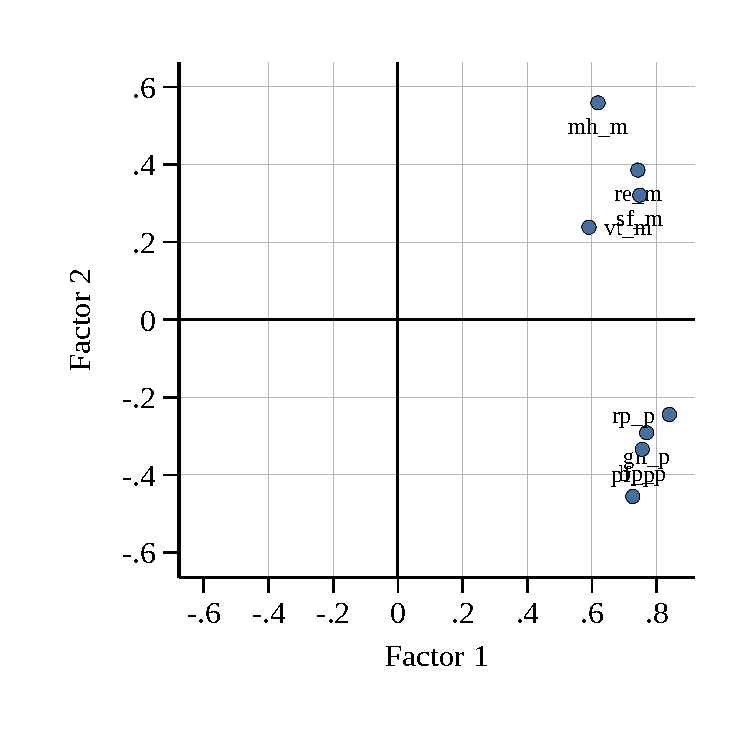
\includegraphics[width=.9\linewidth]{../../output/figures/factor/factor_loadings_norotate.pdf}
        \label{sfig:factorloadingsnorotate}
    \end{subfigure}\\
    \begin{subfigure}{.5\textwidth}\centering
        \caption{SOEP's default (SF-12)\\PCA followed by varimax rotation\\(with Kaiser normalization)}
        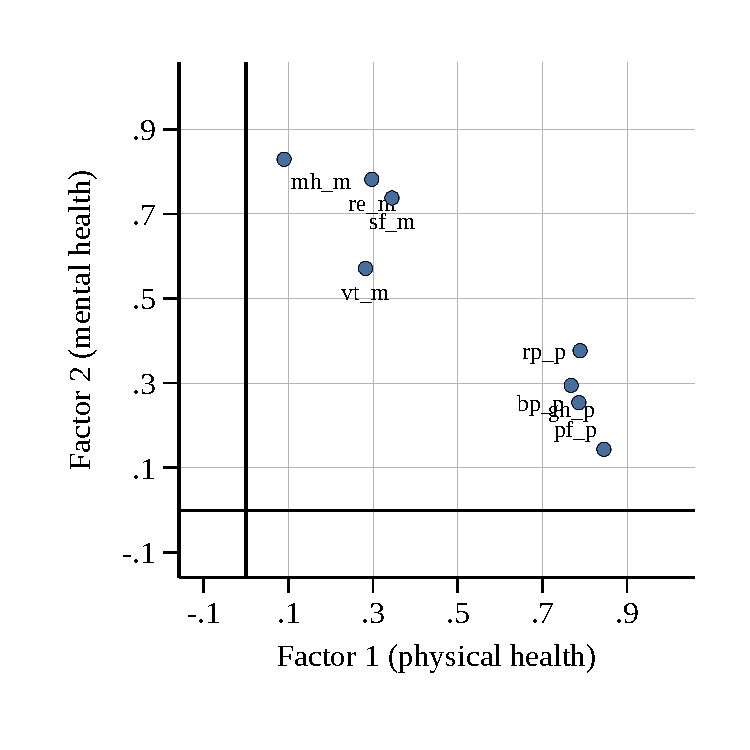
\includegraphics[width=.9\linewidth]{../../output/figures/factor/factor_loadings_a_soeps_default.pdf}
        \label{sfig:factorloadingsdef}
    \end{subfigure}%
    \begin{subfigure}{.5\textwidth}\centering
        \caption{Alternative method\\Principal factors with oblique rotation\\(promax=1.6)}
        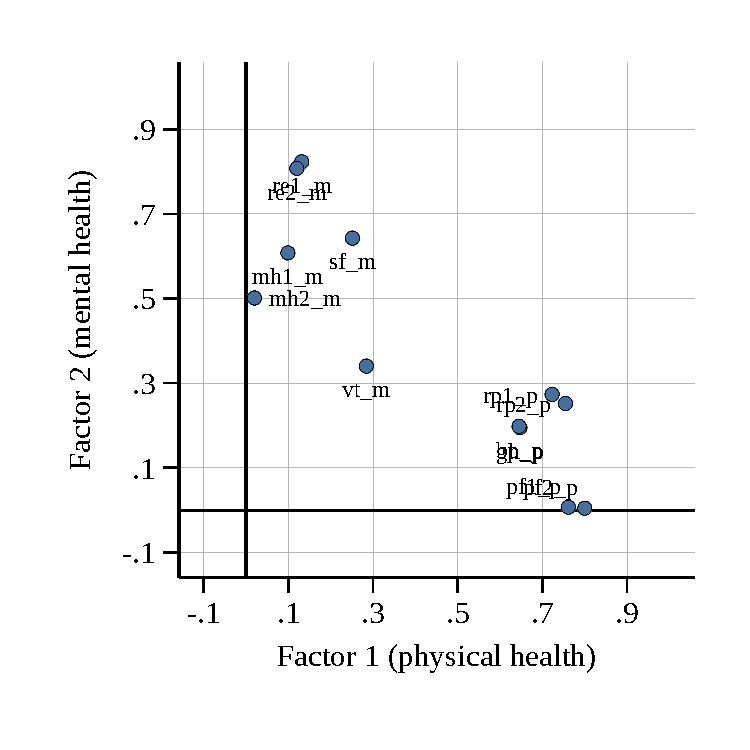
\includegraphics[width=.9\linewidth]{../../output/figures/factor/factor_loadings_b_oblique_main_raw_input_vars.pdf}
        \label{sfig:factorloadingmain}
    \end{subfigure}%
    \caption[Factor loadings comparison between SF-12 and alternative methods]
    {Factor loadings comparison between SF-12 and alternative methods} 
    \label{fig:factorloadings}
    \fnote{
    Notes: The graphs show in both versions that the variables are meaningfully clustered in their
    respective group and the clusters are well separated. However, allowing for an oblique rotation
    results in a clearer factor separation. The loadings of each variable are closer to one of the
    axes, indicating that a variable strongly affects one but not the other factor. 
    Further, by using all variables instead of the mean of grouped variables in the alternative model
    we can confirm that variables from the same category are indeed closely clustered. One drawback
    with the alternative model is that \code{vt} (Vitality) is only weakly loaded from both factors.
    Variables with suffix \textit{m} belong to the mental domain, whereas those with \textit{p} to the physical one. 
    For an overview on the variables see \cref{tab:health_fact_varname_and_questions}. 
    }
\end{figure}



\begin{figure}[tbhp!]
    \begin{subfigure}{.5\textwidth}\centering
        \includegraphics[width=.9\linewidth]{factor/fig_bidim_marg_def.pdf}
        \caption{SF-12 methodology}
        \label{sfig:dens_def}
    \end{subfigure}%
    \begin{subfigure}{.5\textwidth}\centering
        \includegraphics[width=.9\linewidth]{factor/fig_bidim_marg_main.pdf}
        \caption{Alternative methodology}
        \label{sfig:dens_main}
    \end{subfigure}
    \caption[Bivariate density of mental and physical health scores]
    {Bivariate density estimation of mental and physical health scores} \par \footnotesize
    \vspace{5pt} 
    Note: This figure plots the health scores of each individual and shows a bi-variate density on the canvas and a 
    histogram of each domain on the opposite axis. Each point depicts the pcs (x-axis) and mcs (y-axis) for each
    individual. In panel \subref{sfig:dens_def}, the SF-12 methodology is shown and, in \subref{sfig:dens_main}, an
    alternative procedure with oblique rotation. In both methods scores are shifted and scaled to have a 
    mean of 50 and a standard deviation of 10.
    \label{fig:main_bivariate_density}
\end{figure}




% -------------------------------------------------------------------------------------------------
% -------------------------------------------------------------------------------------------------
% part 2 ----
% -------------------------------------------------------------------------------------------------
% -------------------------------------------------------------------------------------------------


















%\clearpage{\pagestyle{empty}\cleardoublepage}